\documentclass[fleqn]{article}
\usepackage[nodisplayskipstretch]{setspace}
\usepackage{amsmath, nccmath}
\usepackage{amssymb}
\usepackage{enumitem}
\usepackage{etoolbox}
\usepackage{scalerel}
\usepackage{graphicx}
\usepackage{float}
\usepackage{changepage}
\usepackage{environ,capt-of}

\newcommand{\zerodisplayskip}{
	\setlength{\abovedisplayskip}{0pt}%
	\setlength{\belowdisplayskip}{0pt}%
	\setlength{\abovedisplayshortskip}{0pt}%
	\setlength{\belowdisplayshortskip}{0pt}%
	\setlength{\mathindent}{0pt}}

\makeatletter
	\newenvironment{equationCenter}{\@fleqnfalse\begin{equation*}}{\end{equation*}}
\makeatother

\makeatletter
	\newenvironment{singleSpaceEquation}{\setlength{\lineskip}{0pt}\vspace{12pt}\begin{equation*}\begin{aligned}}{\end{aligned}\end{equation*}}
\makeatother

\newcommand{\longdiv}{\smash{\mkern-0.43mu\vstretch{1.31}{\hstretch{.7}{)}}\mkern-5.2mu\vstretch{1.31}{\hstretch{.7}{)}}}}

\let\oldfigure\figure% Store original figure float environment
\let\endoldfigure\endfigure
\RenewEnviron{figure}[1][H]{% Update figure environment
  %\par\vspace{\intextsep}% Assume in-text placement, so insert appropriate vertical spacing
  \noindent
  % \patchcmd{<cmd>}{<search>}{<replace>}{<success>}{<failure>}
  \patchcmd{\BODY}{\caption}{\captionof{figure}}{}{}% Replace \caption with \captionof{figure} inside \BODY
  % Set "figure"
  \begin{minipage}{\linewidth}
    \BODY
  \end{minipage}
  %\par\vspace{\intextsep}% Assume in-text placement, so insert appropriate vertical spacing
}

\title{Homework 4}
\author{Owen Sowatzke}
\date{October 24, 2023}
\setlength{\jot}{0pt}

\begin{document}
	\offinterlineskip
	\setlength{\lineskip}{12pt}
	\zerodisplayskip
	\maketitle
	\begin{enumerate}[nolistsep]
		\item[3.8] The system function of a causal LTI system is
	
		\begin{equationCenter}
			H(z) = \frac{1 - z^{-1}}{1 + \frac{3}{4}z^{-1}}
		\end{equationCenter}
		
		The input to this system is
		
		\begin{equationCenter}
			x[n] = \left(\frac{1}{3}\right)^nu[n] + u[-n-1]
		\end{equationCenter}
		
		\begin{enumerate}[nolistsep]
			\item Find the impulse response of the system, $h[n]$.
			
			We can find the impulse response, by taking the inverse z-transform of $H(z)$. However, before taking the inverse z-transform, we must first identify the ROC of $H(z)$.
			
			Because the system is casual, it must also be right-sided. Therefore, the ROC of its z-transform extends outward from
the outermost (largest magnitude) finite pole (i.e. ROC: $|z| > \frac{3}{4}$).

			If we expand the numerator of $H(z)$, we can see how it maps to the z-transform pairs in the table.
			
			\begin{equation*}
				H(z) = \frac{1}{1 + \frac{3}{4}z^{-1}} - \frac{z^{-1}}{1 + \frac{3}{4}z^{-1}},\ \text{ROC:}\ |z| > \frac{3}{4}
			\end{equation*}
			
			\begin{equation*}
				a^nu[n] \leftrightarrow \frac{1}{1 - az^{-1}},\ \text{ROC:}\ |z| > |a| 
			\end{equation*}
			
			\begin{equation*}
				a^{(n-1)}u[n-1] \leftrightarrow \frac{z^{-1}}{1 - az^{-1}},\ \text{ROC:}\ |z| > |a| 
			\end{equation*}
			
			\begin{equation*}
				\mathbf{\therefore h[n] = \left(-\frac{3}{4}\right)^nu[n] - \left(-\frac{3}{4}\right)^{(n-1)}u[n-1]}
			\end{equation*}
			
			\item Find the output $y[n]$.
				
				The z-transform of $y[n]$ can be written as follows:
				
				$Y(z) = H(z)X(z)$.
				
				We can find $X(z)$ using the table of z-transform pairs.
				
				\begin{equation*}
					a^nu[n] \leftrightarrow \frac{1}{1 - az^{-1}},\ \text{ROC:}\ |z| > |a| 
				\end{equation*}
			
				\begin{equation*}
					-u[-n-1] \leftrightarrow \frac{1}{1 - z^{-1}},\ \text{ROC:}\ |z| < 1 
				\end{equation*}
				
				\begin{equation*}
					\therefore X(z) = \frac{1}{1 - \frac{1}{3}z^{-1}} - \frac{1}{1 - z^{-1}} = \frac{1 - z^{-1} - \left(1 - \frac{1}{3}z^{-1}\right)}{\left(1 - \frac{1}{3}z^{-1}\right)\left(1 - z^{-1}\right)}
				\end{equation*}
				
				\begin{equation*}
					= \frac{-\frac{2}{3}z^{-1}}{\left(1 - \frac{1}{3}z^{-1}\right)\left(1 - z^{-1}\right)},\ \text{ROC:}\ \frac{1}{3} < |z| < 1 
				\end{equation*}
				
				\begin{equation*}
					Y(z) = \frac{-\frac{2}{3}z^{-1}(1 - z^{-1})}{\left(1 - \frac{1}{3}z^{-1}\right)\left(1 - z^{-1}\right)\left(1 + \frac{3}{4}z^{-1}\right)}
				\end{equation*}
				
				\begin{equation*}
					= \frac{-\frac{2}{3}z^{-1}}{\left(1 - \frac{1}{3}z^{-1}\right)\left(1 + \frac{3}{4}z^{-1}\right)},\ \text{ROC:}\ |z| > \frac{3}{4} 
				\end{equation*}
				
				Use partial fraction expansion to rewrite $Y(z)$ in a form that we can apply z-transform pairs to.
				
				\begin{equation*}
					\frac{-\frac{2}{3}z^{-1}}{\left(1 - \frac{1}{3}z^{-1}\right)\left(1 + \frac{3}{4}z^{-1}\right)} = \frac{A}{1 - \frac{1}{3}z^{-1}} + \frac{B}{1 + \frac{3}{4}z^{-1}}
				\end{equation*}
				
				\begin{equation*}
					A = \left.\frac{-\frac{2}{3}z^{-1}}{1 + \frac{3}{4}z^{-1}}\right\vert_{z = \frac{1}{3}} = \frac{-\frac{2}{3}(3)}{1 + \frac{3}{4}(3)} = -\frac{2}{1 + \frac{9}{4}} = -\frac{8}{4 + 9} = -\frac{8}{13}
				\end{equation*}
					
				\begin{equation*}
					B = \left.\frac{-\frac{2}{3}z^{-1}}{1 - \frac{1}{3}z^{-1}}\right\vert_{z = -\frac{3}{4}} = \frac{-\frac{2}{3}\left(-\frac{4}{3}\right)}{1 - \frac{1}{3}\left(-\frac{4}{3}\right)} = \frac{\frac{8}{9}}{1 + \frac{4}{9}} = \frac{8}{4 + 9} = \frac{8}{13}
				\end{equation*}
				
				\pagebreak
				\begin{equation*}
					Y(z) = \frac{-\frac{8}{13}}{1 - \frac{1}{3}z^{-1}} + \frac{\frac{8}{13}}{1 + \frac{3}{4}z^{-1}},\ \text{ROC:}\ |z| > \frac{3}{4}
				\end{equation*}
				
				We can now use the following z-transform pair to derive $y[n]$:
				
				\begin{equation*}
					a^nu[n] \leftrightarrow \frac{1}{1 - az^{-1}},\ \text{ROC:}\ |z| > |a| 
				\end{equation*}
				
				\begin{equation*}
					\mathbf{\therefore y[n] = -\frac{8}{13}\left(\frac{1}{3}\right)^nu[n] + \frac{8}{13}\left(-\frac{3}{4}\right)^nu[n]}
				\end{equation*}
				
				
			\item Is the system stable? That is, is $h[n]$ absolutely summable?
			
				The ROC of $H(z)$ includes the unit circle.
				
				\textbf{$\mathbf{\therefore}$ the system is stable.}
		\end{enumerate}
		
				
		\item [3.10] Without explicitly solving for $X(z)$ find the ROC of the z-transform of each of the following sequences, and determine whether the Fourier transform converges:
		
			\begin{enumerate}[nolistsep]
				\item [(b)]

					\begin{equation*}				
						x[n] = \left\{\begin{aligned} 1,& \ -10 \leq n \leq 10, \\ 
						0,& \ \text{otherwise}, \end{aligned}\right.
					\end{equation*}
					
					$x[n]$ is a finite duration signal, so its ROC will be all of $z$ except possibly $z = 0$ or $z = \infty$.
					
					The non-zero $x[n]$ samples for $n > 0$ will create poles at $0$, and the non-zero $x[n]$ samples for $n < 0$ will create poles at $\infty$.
					
					\textbf{$\mathbf{\therefore}$ the ROC of the z-transform will be all of $\mathbf{z}$ except for $\mathbf{z=0}$ and $\mathbf{z=\infty}$. Because the unit circle is contained within the ROC of $\mathbf{X(z)}$, the Fourier Transform converges.}
					
				\item[(f)] $x[n] = \left(\frac{1}{2}\right)^{n-1}u[n] + (2 + 3j)^{n-2}u[-n-1]$
				
				Let $X_1(z) = \left(\frac{1}{2}\right)^{n-1}u[n]$
				
				$X_1(z) \propto \left(\frac{1}{2}\right)^{n}u[n]$.
				
				$\therefore X_1(z)$ has a ROC of $|z| > \frac{1}{2}$
				
				Let $X_2(z) = (2 + 3j)^{n-2}u[-n-1]$
				
				$X_2(z) \propto (2 + 3j)^{n}u[-n-1]$.
				
				$\therefore X_2(z)$ has a ROC of $|z| < |2 + 3j| = \sqrt{13}$
				
				If we denote $R_{X_1}$ as the ROC of $X_1(z)$ and $R_{X_2}$ as the ROC of $X_2(z)$, the ROC of $X_1(z) + X_2(z)$ contains $R_{X_1} \cap R_{X_2}$. If there is no pole-zero cancellation, the ROC of $X_1(z) + X_2(z)$ is exactly $R_{X_1} \cap R_{X_2}$.
				
				If we were to simplify the expressions for $X_1(z) + X_2(z)$, we would find the zeros of the expression and conclude that there is no pole-zero cancellation.
				
				\textbf{$\mathbf{\therefore}$ the ROC of the z-transform will be $\mathbf{\frac{1}{2} < |z| < \sqrt{13}}$. Because the unit circle is contained within the ROC of $\mathbf{X(z)}$, the Fourier Transform converges.}
			\end{enumerate}
			
		\item[3.21] A causal LTI system has the following system function:
		
			\begin{equationCenter}
				H(z) = \frac{4 + 0.25z^{-1}-0.5z^{-2}}{(1-0.25z^{-1})(1 + 0.5z^{-1})}
			\end{equationCenter}
		
			\begin{enumerate}[nolistsep]
				\item[(a)] What is the ROC for $H(z)$?
				
					Because the system is casual, it must also be right-sided. Therefore, the ROC of its z-transform extends outward from
the outermost (largest magnitude) finite pole.

					\textbf{$\mathbf{\therefore}$ ROC is $\mathbf{|z| > 0.5}$}
					
				\item[(b)] Determine if the system is stable or not.
					The ROC of $H(z)$ includes the unit circle.
				
					\textbf{$\mathbf{\therefore}$ the system is stable.}
				 
				 \item[(c)] Determine the difference equation that is satisfied by the input $x[n]$ and the output $y[n]$.
				 
				 	\begin{equation*}
				 		H(z) = \frac{Y(z)}{X(z)} = \frac{4 + 0.25z^{-1}-0.5z^{-2}}{(1-0.25z^{-1})(1 + 0.5z^{-1})}
				 	\end{equation*}
				 	
				 	$Y(z)(1-0.25z^{-1})(1 + 0.5z^{-1}) = X(z)(4 + 0.25z^{-1}-0.5z^{-2})$
				 	
				 	$Y(z)(1 + 0.25z^{-1} - 0.125z^{-2}) = X(z)(4 + 0.25z^{-1}-0.5z^{-2})$
				 	
				 	$Y(z) + 0.25Y(z)z^{-1} - 0.125Y(z)z^{-2}$
				 	
				 	$= 4X(z) + 0.25X(z)z^{-1}-0.5X(z)z^{-2}$
				 	
				 	Take the inverse z-transform of both sides of the equation.
				 	
				 	$y[n] + 0.25y[n-1] - 0.125y[n-2] = 4x[n] + 0.25x[n-1] - 0.5x[n-2]$
				 	
				 	Rearrange the terms to obtain a difference equation for $y[n]$
				 	
				 	$\mathbf{y[n] = -0.25y[n-1] + 0.125y[n-2]}$
				 	
				 	$\mathbf{ + 4x[n] + 0.25x[n-1] - 0.5x[n-2]}$
				 	
				 \item[(d)] Use a partial fraction expansion to determine the impulse response $h[n]$.
				 
				 	\begin{equation*}
				 		H(z) = \frac{4 + 0.25z^{-1}-0.5z^{-2}}{(1-0.25z^{-1})(1 + 0.5z^{-1})} = \frac{4 + 0.25z^{-1}-0.5z^{-2}}{1 + 0.25z^{-1} - 0.125z^{-2}}
				 	\end{equation*}
				 	
				 	For partial fraction expansion to work, the numerator degree of $H(z)$ must be less than the denominator degree. Because this is not the case for $H(z)$, we must first rewrite $H(z)$ in a form that satisfies this criteria. This can be done use long division as shown below:
						
					\[
					\arraycolsep=1pt
					\renewcommand\arraystretch{1.2}
					\begin{array}{*1r @{\hskip\arraycolsep}c@{\hskip\arraycolsep} *{11}r}
        				& & 4 & & & & & \\
					\cline{2-7}
					1 + 0.25z^{-1} - 0.125z^{-2} & \longdiv & 4 & + & 0.25z^{-1} & - & 0.5z^{-2}\\
        				& & 4 & + & z^{-1} & - & 0.5z^{-2} & & & \\
					\cline{3-7}
        				& & & - & 0.75z^{-1} & & & &
					\end{array}
					\]
					
					\begin{equation*}
						\therefore H(z) = 4 - \frac{0.75z^{-1}}{1 + 0.25z^{-1} - 0.125z^{-2}}
					\end{equation*}
					
					\begin{equation*}
						= 4 - \frac{0.75z^{-1}}{(1 - 0.25z^{-1})(1 + 0.5z^{-1})}
					\end{equation*}
					
					\pagebreak
					Note that the numerator degree of the fractional term is now less than the denominator degree. As such, we can expand the fractional term using partial fractional expansion.
					
					\begin{equation*}
						\frac{0.75z^{-1}}{(1 - 0.25z^{-1})(1 + 0.5z^{-1})} = \frac{A}{1 - 0.25z^{-1}} + \frac{B}{1 + 0.5z^{-1}}
					\end{equation*}
					
					\begin{equation*}
				 		A = \left.\frac{0.75z^{-1}}{1 + 0.5z^{-1}}\right\vert_{z = 0.25} = \frac{0.75(4)}{1 + 0.5(4)} = \frac{3}{3} = 1
				 	\end{equation*}
				 	
				 	\begin{equation*}
				 		B = \left.\frac{0.75z^{-1}}{1 - 0.25z^{-1}}\right\vert_{z = -0.5} = \frac{0.75(-2)}{1 - 0.25(-2)} = -\frac{1.5}{1.5} = -1
				 	\end{equation*}
					
					\begin{equation*}
						\therefore H(z) = 4 - \left(\frac{1}{1-0.25z^{-1}} - \frac{1}{1+0.5z^{-1}}\right)
					\end{equation*}
					
					\begin{equation*}
						= 4 - \frac{1}{1-0.25z^{-1}} + \frac{1}{1+0.5z^{-1}}
					\end{equation*}
					
					We can now take the inverse z-transform of $H(z)$ using a table of z-transform pairs.
					
					\begin{equation*}
						\mathbf{h[n] = 4\delta[n] - \left(\frac{1}{4}\right)^nu[n] + \left(-\frac{1}{2}\right)^nu[n]}
					\end{equation*}
					
				\end{enumerate}
				
			\item[3.40] If the input $x[n]$ to an LTI system is $x[n] = u[n]$, the output is
				
				\begin{equationCenter}
					y[n] = \left(\frac{1}{2}\right)^{n-1}u[n+1]
				\end{equationCenter}
					
				\begin{enumerate}[nolistsep]
					\item[(a)] Find $H(z)$, the z-transform of the system impulse response, and plot its pole-zero diagram.
					
						\begin{equation*}
							y[n] = \left(\frac{1}{2}\right)^{-2}\left(\frac{1}{2}\right)^{n+1}u[n+1] = 4\left(\frac{1}{2}\right)^{n+1}u[n+1]
						\end{equation*}
						
						\begin{equation*}
							\Rightarrow Y(z) = \frac{4z}{1 - \frac{1}{2}z^{-1}}\quad \text{ROC:}\ |z| > \frac{1}{2}
						\end{equation*}
						
						\begin{equation*}
							\Rightarrow X(z) = \frac{1}{1 - z^{-1}} \quad \text{ROC:}\ |z| > 1
						\end{equation*}
						
						\begin{equation*}
							H(z) = \frac{Y(z)}{X(z)} = \frac{4z(1 - z^{-1})}{1 - \frac{1}{2}z^{-1}}
						\end{equation*}
						
						Because the input and output of the system are both right-sided, we know that the impulse response must be right-sided as well. As such, the ROC of $H(z)$ extends outward from
the outermost (largest magnitude) finite pole.
					
						\begin{equation*}
							\mathbf{\therefore H(z) = \frac{Y(z)}{X(z)} = \frac{4z(1 - z^{-1})}{1 - \frac{1}{2}z^{-1}}\quad \text{\textbf{ROC:}}\ |z| > \frac{1}{2}}
						\end{equation*}
						
						\begin{figure}[H]				
						\centerline{\fbox{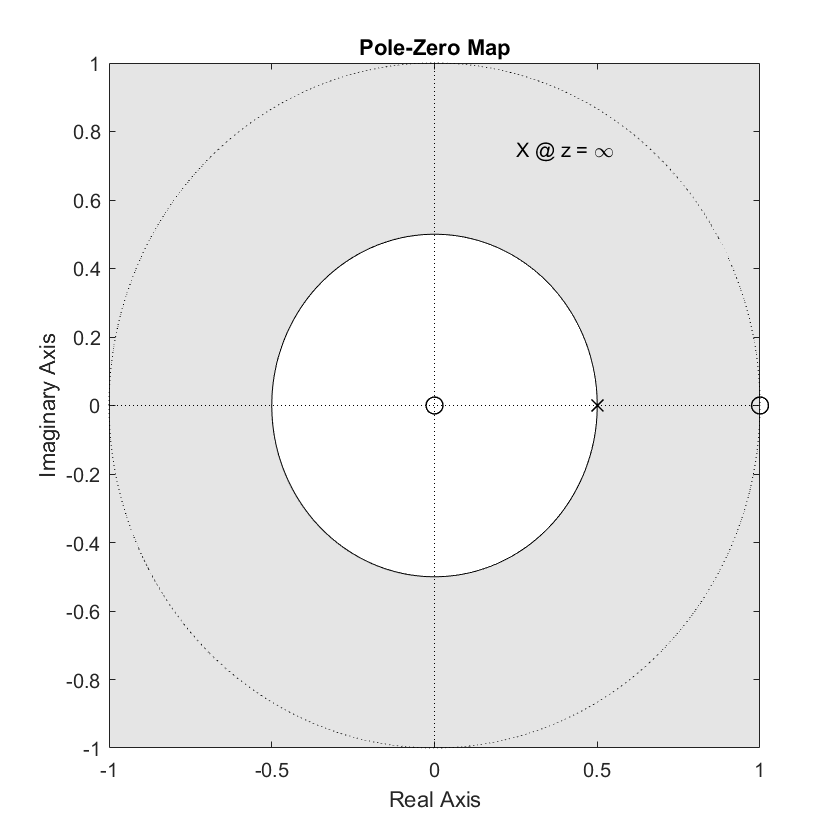
\includegraphics[width=0.5\textwidth]{pzmap_prob_3_40.png}}}
						\caption{Pole-Zero Map of H(z)}
						\label{pzmap_prob_3_40}
						\end{figure}
						
					\item[(b)] Find the impulse response $h[n]$.
					
						\begin{equation*}
							H(z) = \frac{4z(1 - z^{-1})}{1 - \frac{1}{2}z^{-1}} = \frac{4z - 4}{1 - \frac{1}{2}z^{-1}} = \frac{4z}{1 - \frac{1}{2}z^{-1}} - \frac{4}{1 - \frac{1}{2}z^{-1}}
						\end{equation*}
						
						Take the inverse z-transform of $H(z)$ using a table of z-transform pairs.
						
						\begin{equation*}
							h[n] = 4\left(\frac{1}{2}\right)^{n+1}u[n+1] - 4\left(\frac{1}{2}\right)^{n}u[n]
						\end{equation*}
						
						\begin{equation*}
							\Rightarrow h[n] = 4\delta[n+1] + 4\left(\frac{1}{2}\right)^{n+1}u[n] - 4\left(\frac{1}{2}\right)^{n}u[n]
						\end{equation*}
						
						\begin{equation*}
							\Rightarrow h[n] = 4\delta[n+1] + 4\left(\frac{1}{2}\right)\left(\frac{1}{2}\right)^{n}u[n] - 4\left(\frac{1}{2}\right)^{n}u[n]
						\end{equation*}
						
						\begin{equation*}
							\Rightarrow h[n] = 4\delta[n+1] + 2\left(\frac{1}{2}\right)^{n}u[n] - 4\left(\frac{1}{2}\right)^{n}u[n]
						\end{equation*}
						
						\begin{equation*}
							\mathbf{\Rightarrow h[n] = 4\delta[n+1] - 2\left(\frac{1}{2}\right)^{n}u[n]}
						\end{equation*}
					
					\item[(c)] Is the system stable?
					
						\textbf{The ROC of $\mathbf{H(z)}$ contains the unit circle, so the system is stable.}
						
					\item[(d)] Is the system causal?
					
						\textbf{Because $\mathbf{h[n]}$ is nonzero at $\mathbf{n = -1}$, the system is not causal. (Note we could have also arrived at this conclusion by noting that there is a pole at $\mathbf{z = \infty}$).}
				\end{enumerate}
				
			\item[3.48] The signal $y[n]$ is the output of an LTI system with impulse response $h[n]$ for a given input $x[n]$. Throughput the problem, assume that $y[n]$ is stable and has a z-transform of $Y(z)$ with the pole-zero diagram shown in Figure \ref{pzmap_y_z_prob_3_48}. The signal $x[n]$ is stable and has the pole-zero diagram shown in Figure \ref{pzmap_x_z_prob_3_48}. 
					
				\begin{figure}[H]				
				\centerline{\fbox{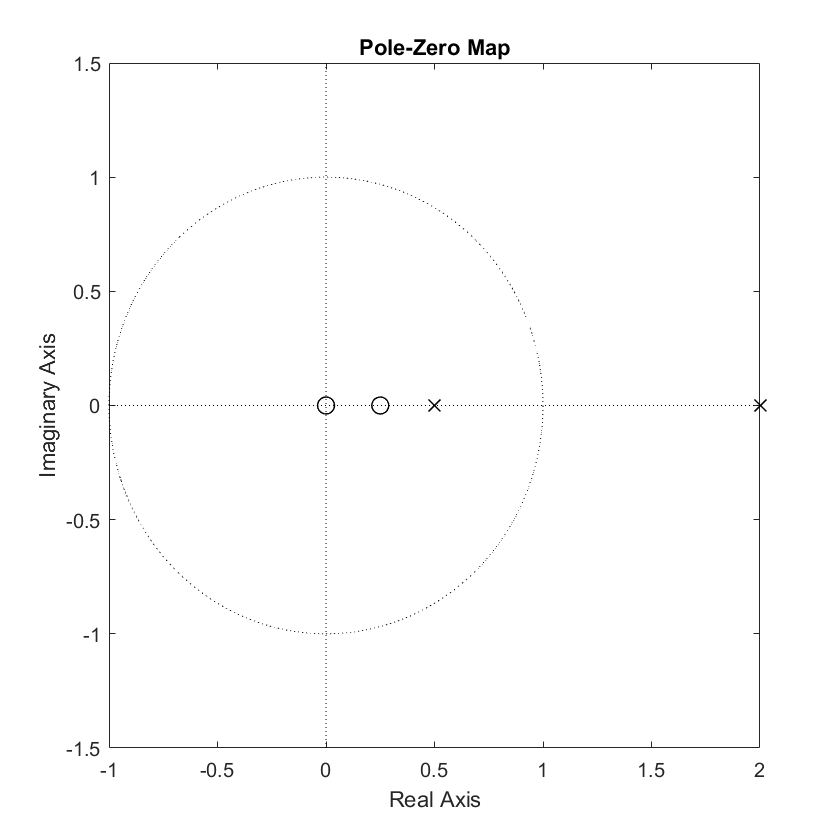
\includegraphics[width=0.5\textwidth]{pzmap_y_z_prob_3_48.png}}}
				\caption{Pole-Zero Map of Y(z)}
				\label{pzmap_y_z_prob_3_48}
				\end{figure}
				
				\begin{figure}[H]				
				\centerline{\fbox{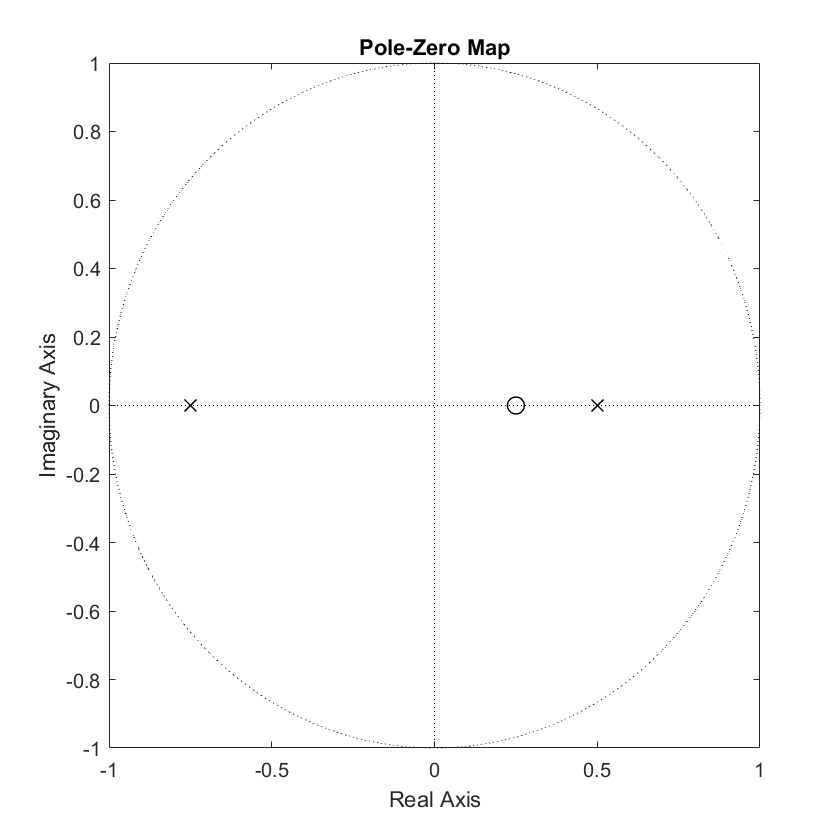
\includegraphics[width=0.5\textwidth]{pzmap_x_z_prob_3_48.png}}}
				\caption{Pole-Zero Map of X(z)}
				\label{pzmap_x_z_prob_3_48}
				\end{figure}
				
				\begin{enumerate} [nolistsep]
					\item[(a)] What is the ROC of $Y(z)$?
					
						For $y[n]$ to be stable, its ROC must contain the unit circle.
						
						\textbf{$\mathbf{\therefore}$ the ROC of $\mathbf{Y(z)}$ must be $\mathbf{\frac{1}{2} < |z| < 2}$.}
						
					\item[(b)] Is $y[n]$ left-sided, right-sided, or two-sided?
					
						The ROC of $Y(z)$ is a ring in the z-plane.
						
						\textbf{$\mathbf{\therefore y[n]}$ is two-sided.}
						
					\item[(c)] What is the ROC of $X(z)$?
					
						For $x[n]$ to be stable, its ROC must contain the unit circle.
						
						\textbf{$\mathbf{\therefore}$ the ROC of $\mathbf{X(z)}$ must be $\mathbf{|z| > \frac{3}{4}}$.}
						
					\item[(d)] Is $x[n]$ a causal sequence? That is, does $x[n] = 0$ for $n < 0$?
					
						Because the ROC of $X(z)$ extends outward from the outermost pole, we know that $x[n]$ must be a right-sided signal.
						
						For a right-sided signal to be causal, it must not have a pole at $z = \infty$.
						
						\textbf{Because $\mathbf{X(z)}$ does not have a pole at $\mathbf{z = \infty}$, $\mathbf{x[n]}$ must be causal.}
					
					\pagebreak	
					\item[(e)] What is $x[0]$?
					
						Because $x[n]$ is causal. $x[0] = \displaystyle\lim_{z\to\infty}{X(z)}$
						
						\begin{equation*}
							X(z) = \frac{A\left(z - \frac{1}{4}\right)}{\left(z - \frac{1}{2}\right)\left(z - \frac{3}{4}\right)}
						\end{equation*}
						
						\begin{equation*}
							\mathbf{x[0] = \displaystyle\lim_{n\to\infty}{X(z)} = \displaystyle\lim_{z\to\infty}{\frac{A\left(z - \frac{1}{4}\right)}{\left(z - \frac{1}{2}\right)\left(z - \frac{3}{4}\right)}} = 0}
						\end{equation*}
							
					\item[(f)] Draw the pole-zero plot of $H(z)$, and specify its ROC.
					
					\begin{equation*}
						H(z) = \frac{Y(z)}{X(z)} = \frac{Bz\left(z - \frac{1}{4}\right)}{\left(z - \frac{1}{2}\right)\left(z - 2\right)}\left(\frac{\left(z - \frac{1}{2}\right)\left(z - \frac{3}{4}\right)}{A\left(z - \frac{1}{4}\right)}\right)
					\end{equation*}
					
					\begin{equation*}
						\Rightarrow H(z) = \frac{Y(z)}{X(z)} = \frac{Bz\left(z - \frac{3}{4}\right)}{A\left(z - 2\right)}
					\end{equation*}
					
					Let $R_X$ specify the ROC of $X(z)$, $R_H$ specify the ROC of $H(z)$, and $R_Y$ specify the ROC of $Y(z)$. $R_H$ must be chosen such that $R_X \cap R_H$ is contained in $R_Y$. 
					
					There are two choices for $R_H$: $|z| < 2$ or $|z| > 2$.
					
					Let $R_H$ be $|z| > 2$, then $R_X \cap R_H$ is $|z| > 2$, which is not contained in $R_Y$. Therefore, $R_H$ is not $|z| > 2$.
					
					Let $R_H$ be $|z| < 2$, then $R_X \cap R_H$ is $\frac{3}{4} < |z| < 2$, which is contained in $R_Y$. Therefore, $R_H$ is $|z| < 2$.
					
					\textbf{The pole-zero diagram of $\mathbf{H(z)}$ is shown in Figure \ref{pzmap_h_z_prob_3_48}. Note that the ROC is $\mathbf{|z| < 2}$.}
					
					\begin{figure}[H]				
					\centerline{\fbox{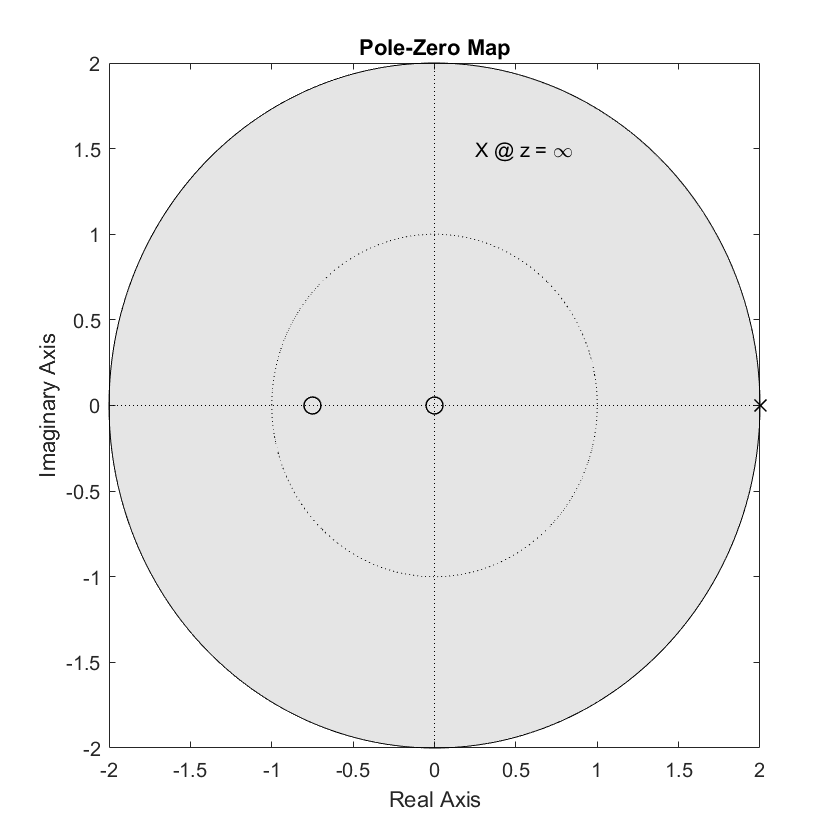
\includegraphics[width=0.5\textwidth]{pzmap_h_z_prob_3_48.png}}}
					\caption{Pole-Zero Map of H(z)}
					\label{pzmap_h_z_prob_3_48}
					\end{figure}
					
				\end{enumerate}
				
			\item[(g)] Is $h[n]$ anticausal? That is does $h[n] = 0$ for $n > 0$?
			
				Any $H(z)$ can be written in the following form:
				
				\begin{equation*}
					H(z) = \sum_{n = -\infty}^{\infty}h(n)z^{-n}
				\end{equation*}
				
				For $h(n)$ to be anticausal, $h(n) = 0$ for $n > 0$. In other words, $H(z)$ should not contain any terms with negative powers of $z$. Because terms with negative powers of $z$ blow up at $z = 0$, we can check whether any of these terms exist by checking if there are any poles at $z = 0$.
				
				Because $H(z)$ has no poles at $z = 0$, $H(z)$ does not contain any negative powers of $z$ and $h[n] = 0$ for $n > 0$.
				
				\textbf{$\mathbf{\therefore h[n]}$ is anticausal.}
	\end{enumerate}
	
\end{document}